\documentclass[a4paper]{article}

%% Language and font encodings
\usepackage[portuges]{babel}
%\usepackage{fontspec}

%% Sets page size and margins
\usepackage[a4paper,top=3cm,bottom=2cm,left=3cm,right=3cm,marginparwidth=1.75cm]{geometry}

%% Useful packages
\usepackage{amsmath,amsthm,amssymb,amsfonts}
\usepackage{graphicx}
\usepackage[colorinlistoftodos]{todonotes}
\usepackage[colorlinks=true, allcolors=blue]{hyperref}
\usepackage{subfig}
\usepackage{float}



\newcommand{\R}{\mathbb{R}}
\newcommand{\N}{\mathbb{N}}
\newcommand{\Z}{\mathbb{Z}}
\providecommand{\C}{\mathbb{C}}

\theoremstyle{definition}
\newtheorem{defin}{Definição}

\theoremstyle{plain}
\newtheorem{theorem}[defin]{Teorema}
\newtheorem{corollary}[defin]{Corolário}



\title{Laboratório de CEME - Lab 2\\Simulação de um sistema eletromecânico: Contatora}

\author{Cleiton M. Freitas\\
}

\date{}

\begin{document}
\maketitle

%\begin{abstract}
%Your abstract.
%\end{abstract}

%%%%%%%%%%%%%%%%%%%%%%%%%%%%%%%%%%%%%%%%%%
%%%%%%%%%%%%%%%%%%%%%%%%%%%%%%%%%%%%%%%%%%
%%%%%%%%%%%%%%%%%%%%%%%%%%%%%%%%%%%%%%%%%%
\section{Objetivo}

O objetivo desta experiência é montar a simulação de um sistema eletromecânico simples, o sistema de uma contatora. Para isso, combinaremos os métodos aprendidos na aula teórica com a metodologia de simulação utilizada no \textbf{LAB 1}.

%%%%%%%%%%%%%%%%%%%%%%%%%%%%%%%%%%%%%%%%%%
%%%%%%%%%%%%%%%%%%%%%%%%%%%%%%%%%%%%%%%%%%
%%%%%%%%%%%%%%%%%%%%%%%%%%%%%%%%%%%%%%%%%%
\section{A contatora}


Uma contatora é um sistema geralmente utilizado como chave eletromecânica. Ou seja, quando injetamos corrente na sua bobina, a parte móvel do núcleo é atraída para uma posição de forma a fechar ou abrir um circuito. Uma boa descrição do funcionamento de uma contatora é encontrada em \cite{Faustino2020} e \cite{meletrica2014}.


A Figura~\ref{fig:contatora} apresenta o diagrama com dois estados de uma contatora similar àquela explicada em \cite{Faustino2020,meletrica2014}. Como pode ser observado, a contatora possui um núcleo dividido em duas partes, uma delas fixa e outra móvel, uma bobina e uma mola. A bobina é enrolada em um carretel, não representado aqui, que serve de suporte para a mola. Assim, o formato da bobina se materá inalterado independentemente da condição da mola. Quando a corrente na bobina é nula, a mola empurra a parte móvel do núcleo para longe da parte fixa. Quando injetamos corrente, a força magnética produzida gera uma atração entre as diferentes partes do núcleo e, consequentemente, a mola é contraída. A Figura~\ref{fig:contatora:comI} apresenta o caso extremo, onde as duas partes do núcleo se tocam, mas a compressão da mola (e a distância entre as partes do núcleo) vai depender da quantidade de corrente injetada na bobina.
%
\begin{figure}[H]
\centering
\subfloat[$i = 0$]{
\label{fig:contatora:semI}
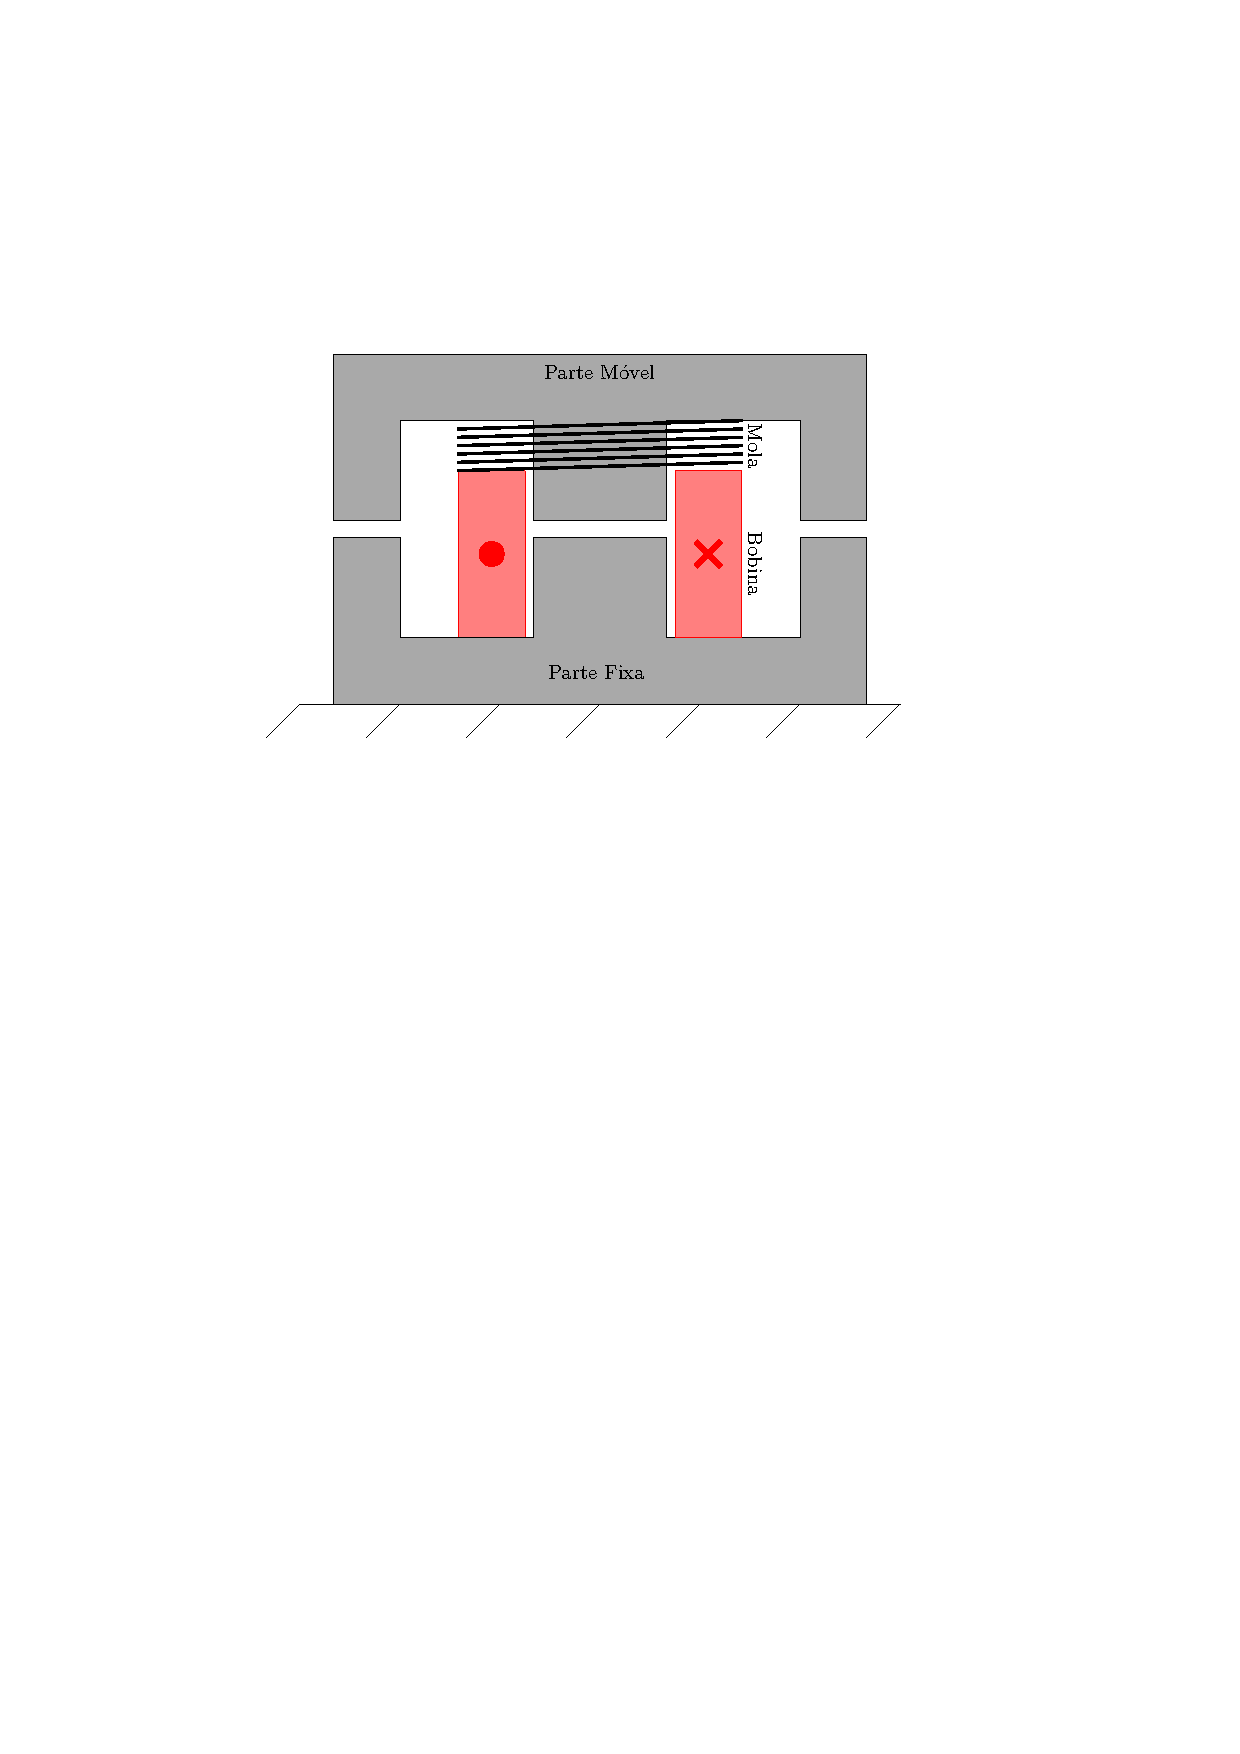
\includegraphics[width=0.48\linewidth]{./figuras/contatora_0}
}
\subfloat[$i \neq 0$]{
\label{fig:contatora:comI}
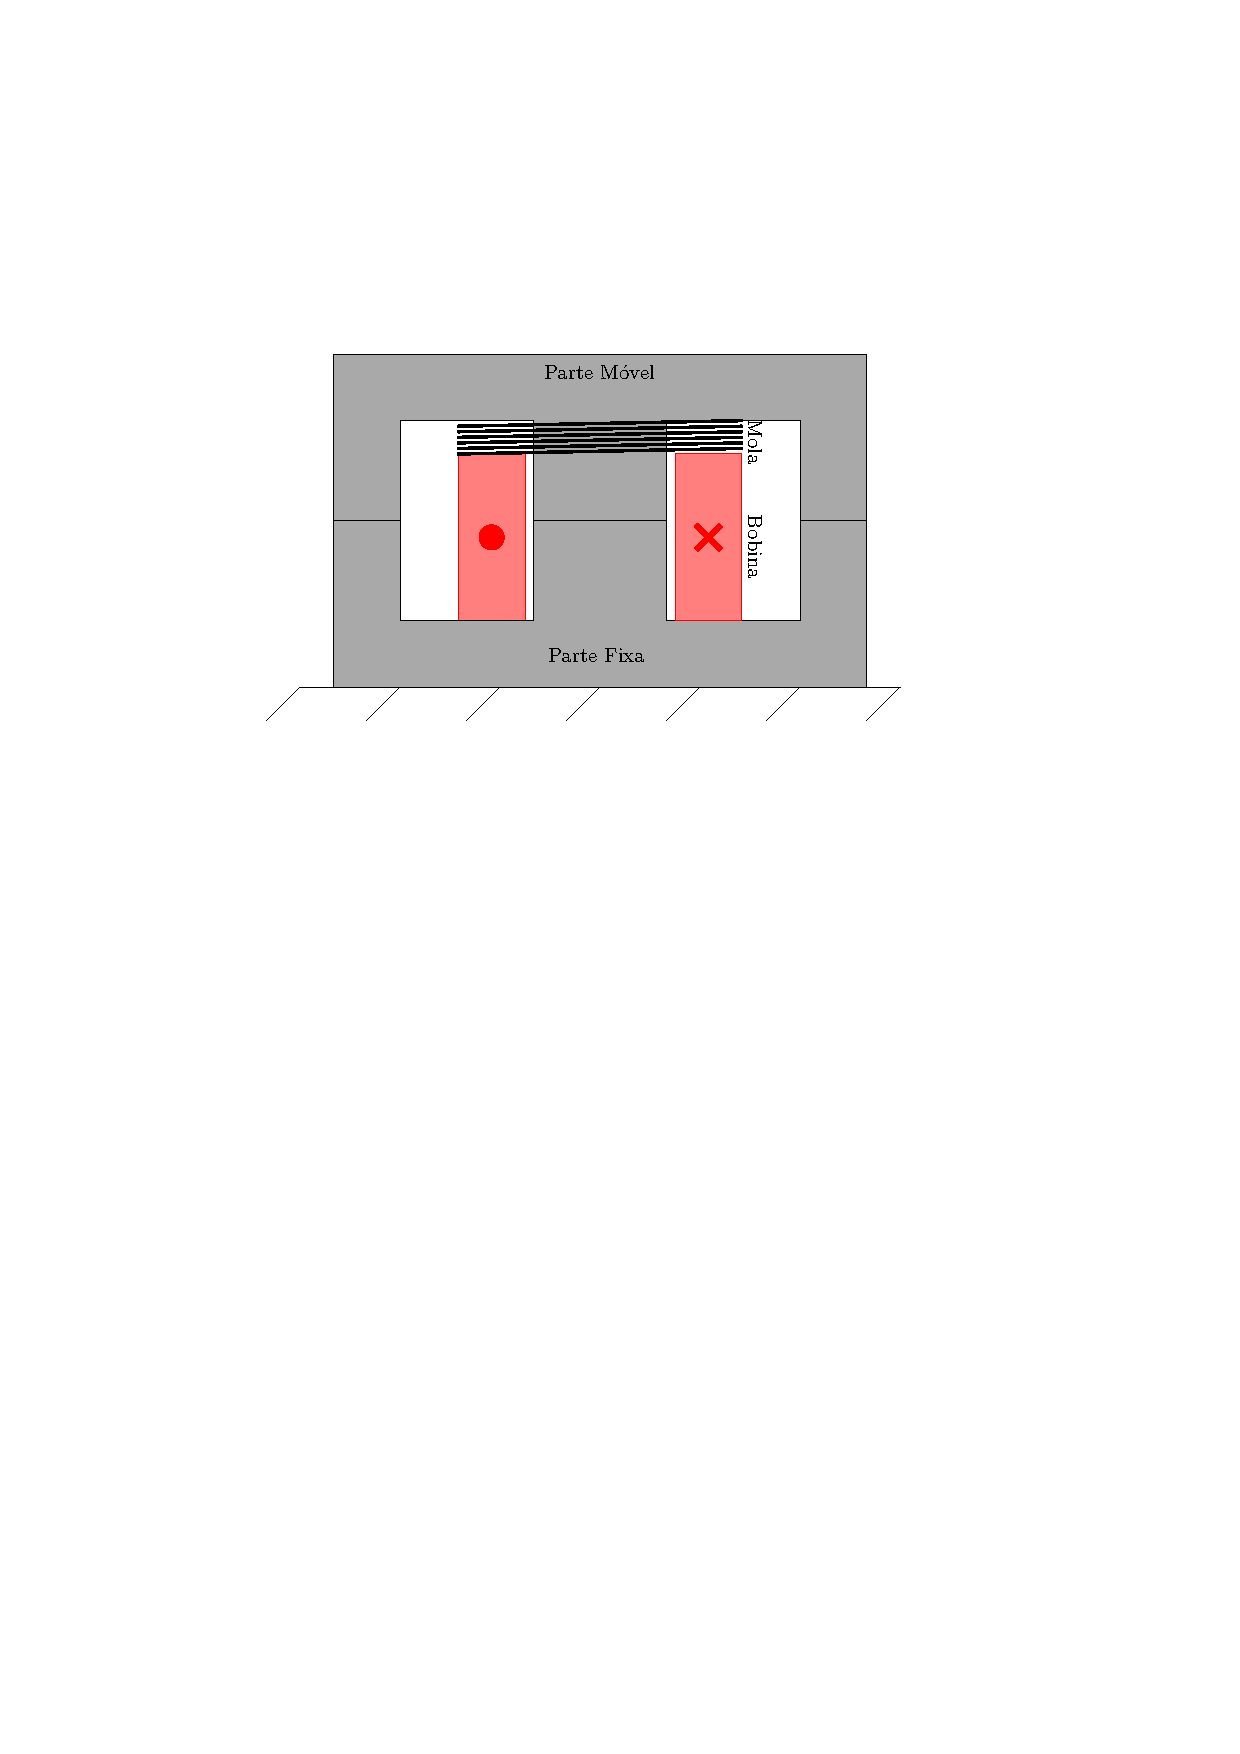
\includegraphics[width=0.48\linewidth]{./figuras/contatora_1}
}
\caption{Esquema de uma contatora}
\label{fig:contatora}
\end{figure}

 


%%%%%%%%%%%%%%%%%%%%%%%%%%%%%%%%%%%%%%%%%%
%%%%%%%%%%%%%%%%%%%%%%%%%%%%%%%%%%%%%%%%%%
%%%%%%%%%%%%%%%%%%%%%%%%%%%%%%%%%%%%%%%%%%
\section{Desenvolvimento das Simulações}


Como no caso anterior, a simulação deverá ser capaz de calcular a resposta dinâmica do sistema para uma conjunto de variáveis. Neste caso, a corrente da bobina ($i$), a posição ($x$) e a velocidade ($v$) da parte móvel do núcleo. A Figura~\ref{fig:cotas} apresenta um novo diagrama da contatora, desta vez omitindo a mola para facilitar a análise da parte magnética. Observe que todos os diagramas representam a vista superior da contatora, ou seja, o sistema está deitado e não sofre atuação da força da gravidade. Além disso, as duas partes do núcleo são simétricas, ou seja, as cotas da parte fixa (inferior) são iguais as da parte móvel (superior).



\begin{figure}[!htb]
\centering
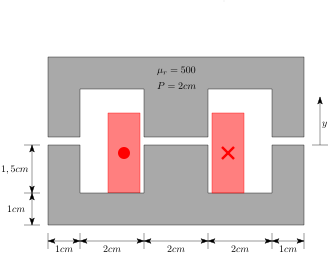
\includegraphics[width=0.85\linewidth]{./figuras/contatora_cotas}
\caption{Diagrama da contatora com as devidas cotas}
\label{fig:cotas}
\end{figure}


Como esperado, para simular a dinâmica do sistema, deveremos obter três equações diferenciais\footnote{Embora tenha escrito $f_1$, $f_2$ e $f_3$ com três variáveis, $x$, $i$ e $v$, nem todas funções terá as três variáveis}:

\begin{equation}
\frac{d i}{dt} = f_1 (x,i,v)
\end{equation}

\begin{equation}
\frac{d x}{dt} = f_2 (x,i,v)
\end{equation}

\begin{equation}
\frac{d v}{dt} = f_3 (x,i,v)
\end{equation}



Para obter a equação diferencial da corrente, devemos seguir um procedimento parecido ao utilizado no \textbf{LAB 1}. Ou seja, devemos obtê-la a partir da manipulação da equação de malha do circuito elétrico da Figura~\ref{fig:mag}. Neste circuito, $V_{in}$ é uma tensão constante que alimentará a bobina e $e$ é a tensão induzida da bobina.


\begin{figure}[!htb]
\centering
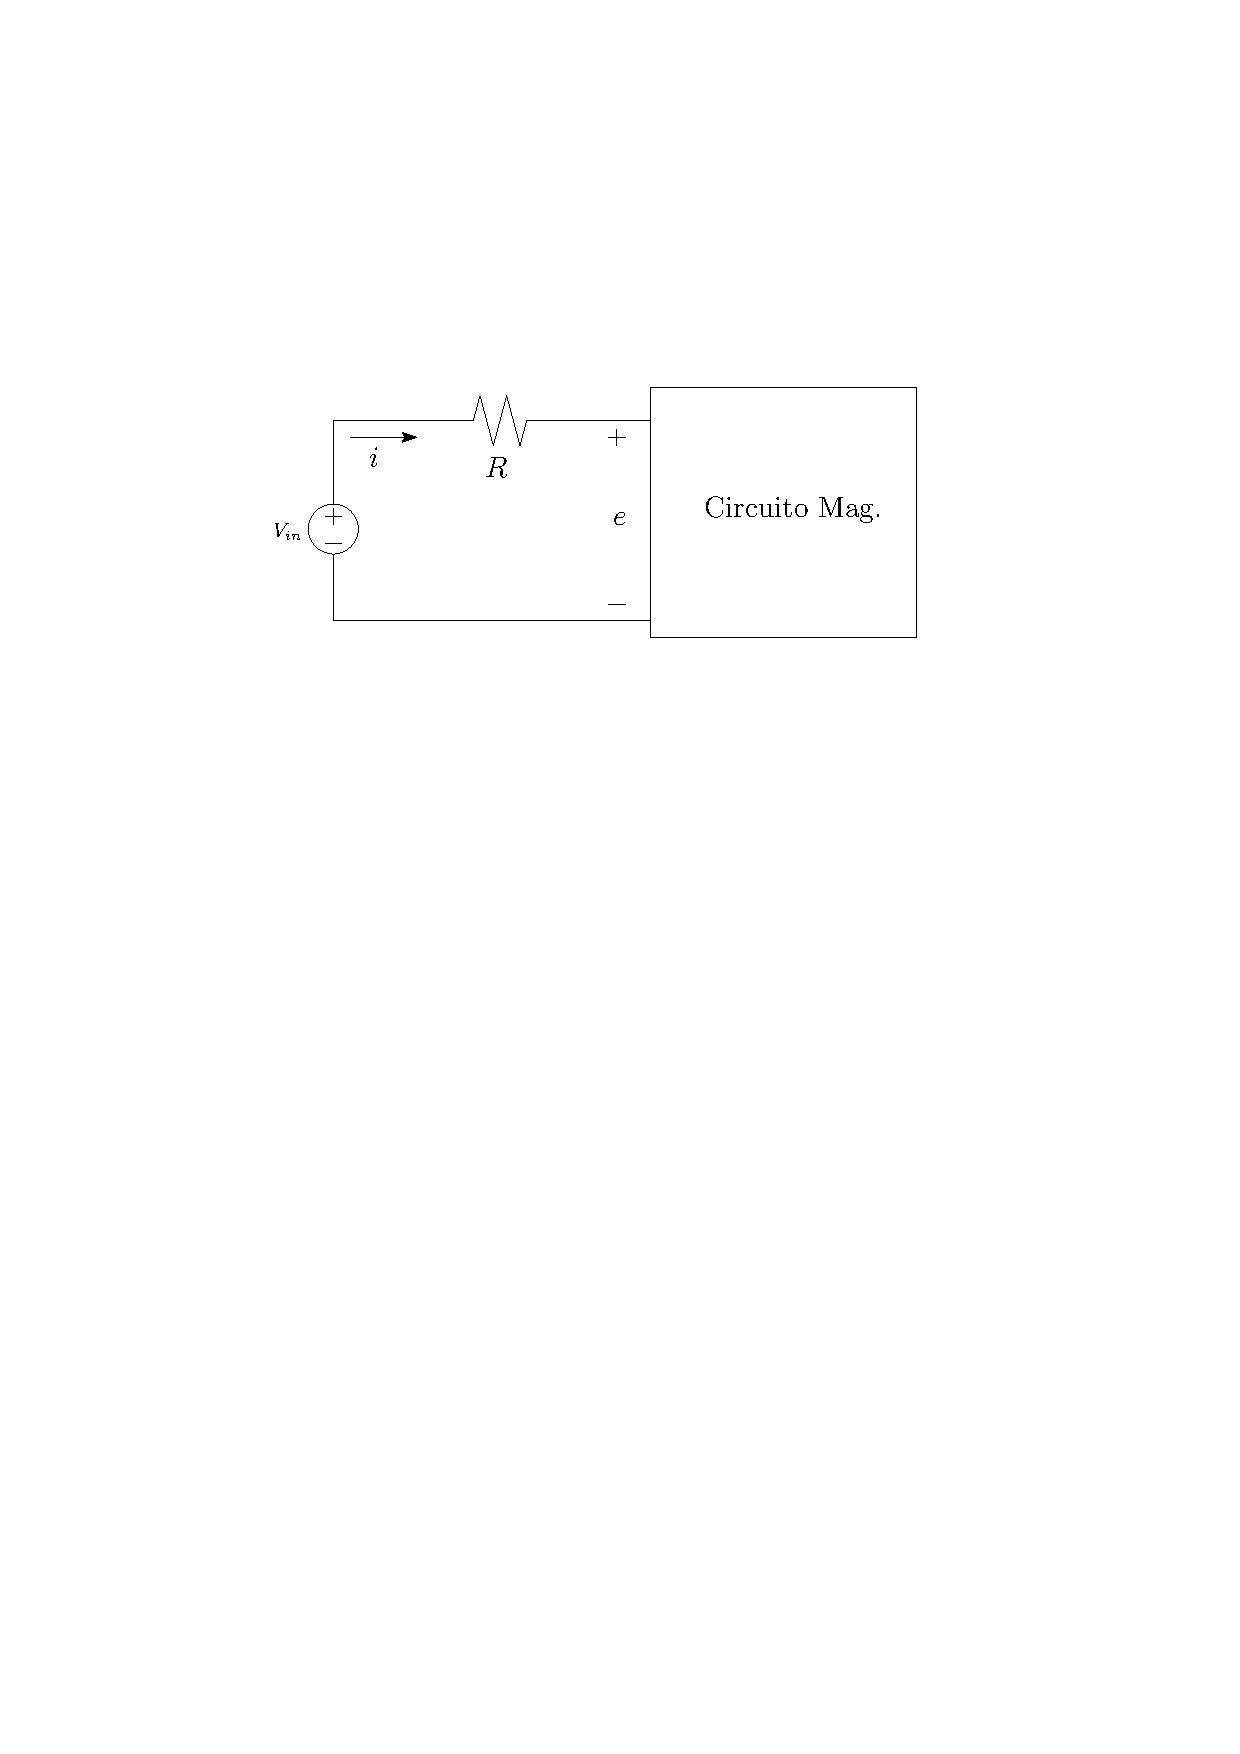
\includegraphics[width=0.50\linewidth]{./figuras/circuito_bobina}
\caption{Interface eletromagnética do sistema}
\label{fig:mag}
\end{figure}


Para obter as equações mecânicas, ou seja, as equações diferenciais de $x$ e $v$, devemos recorrer aos nossos conhecimentos de física básica. Assim:

\begin{equation}
m a = \displaystyle \sum \text{Forças}
\end{equation}
%
onde $m$ e $a$ são a massa e a aceleração da parte móvel. Considerem três forças no sistema, a força magnética, a força da mola e a força do atrito. Lembrem que as equações devem estar em função de $x$, $v$ e $i$. Ou seja, o $a$ não pode aparecer


A equação diferencial de $x$ é direta. 



%%%%%%%%%%%%%%%%%%%%%%%%%%%%%%%%%%%%%%%%%%%
%%%%%%%%%%%%%%%%%%%%%%%%%%%%%%%%%%%%%%%%%%
%%%%%%%%%%%%%%%%%%%%%%%%%%%%%%%%%%%%%%%%%%
\section{Tarefas}


\begin{enumerate}
	\item Obter a indutância do circuito em função da posição $x$ da parte móvel do núcleo.
	\item Calcular a força magnética em função da posição $x$ e da corrente $i$.
	\item Obter a equação diferencial de corrente
	\item Obter a equação diferencial da posição $x$
	\item Obter a equação diferencial da velocidade $v$
\end{enumerate}


%
%A Figura~\ref{fig:trafo:quadri} possui a representação em quadripolo\footnotemark de um transformador monofásicos. Neste circuito, $i_1$ e $i_2$ são as correntes que entram nos enrolamentos primário e secundário do transformador. Além disso, $e_1$ e $e_2$ são as tensões induzidas destes enrolamentos. A caixa nomeada \textbf{Sistema Eletromag.}, por sua vez, representa a interação eletromagnética no circuito. Ou seja, ela representa as seguintes equações:
%
%\begin{equation}
%\begin{bmatrix}
%\lambda_1(t)\\[5pt]
%\lambda_2(t)
%\end{bmatrix} =
%\begin{bmatrix}
%L_{11} & L_{12}\\[5pt]
%L_{21} & L_{22}
%\end{bmatrix}
%\begin{bmatrix}
%i_1(t)\\[5pt]
%i_2(t)
%\end{bmatrix}
%\label{eq:lambda}
%\end{equation} 
%
%
%\begin{equation}
%\begin{bmatrix}
%e_1(t)\\[5pt]
%e_2(t)
%\end{bmatrix} =
%\frac{d}{dt} 
%\begin{bmatrix}
%\lambda_1(t)\\[5pt]
%\lambda_2(t)
%\end{bmatrix}
%\label{eq:e}
%\end{equation}
%
%
%\footnotetext{Deixo como curiosidade a página sobre \href{https://pt.wikipedia.org/wiki/Quadripolo}{quadripolos} na Wikipedia. Este assunto sempre aparece nos últimos capítulos dos livros de circuito, mas por questão tempo nem sempre é abordado em aula.}
%
%\begin{figure}[H]
%\centering
%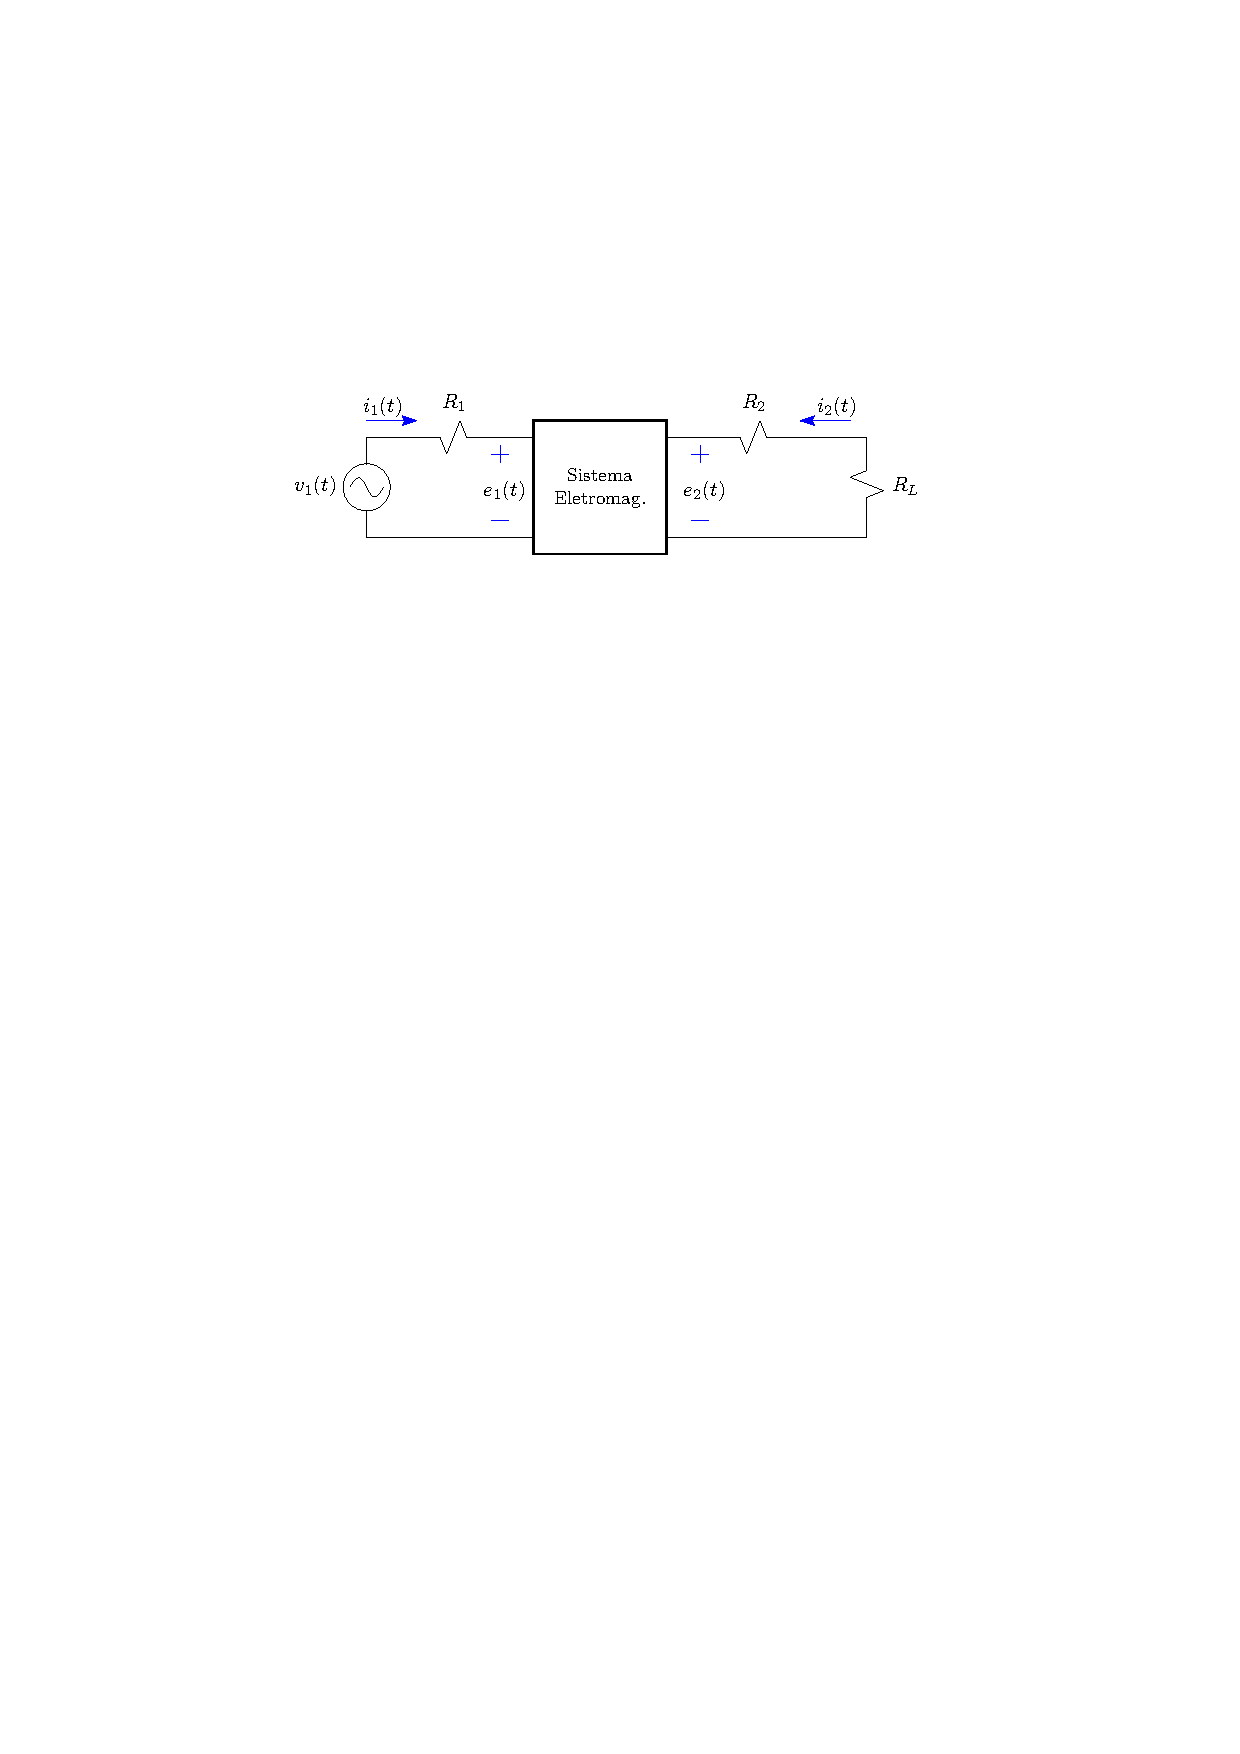
\includegraphics[width=0.75\linewidth]{../../Figuras/Trafo_mono_sistema_eletromag.pdf}
%\caption{Representação em quadripolo do transformador}
%\label{fig:trafo:quadri}
%\end{figure}
%
%
%O circuito ainda apresenta três resistências e uma fonte de tensão. $R_1$ e $R_2$ são as resistências dos enrolamentos e $R_L$ a resistência de carga.  
%
%O primeiro objetivo da simulação é computar as correntes $i_1$ e $i_2$ neste circuito. Para isso, o primeiro passo é obter duas equações diferencias que descrevam estas correntes em função da tensão apicada no primário. Ou seja, obter o seguinte par de equações:
%
%\begin{equation}
%\frac{d i_1}{dt} = f_1(t,v_1, i_1, i_2)
%\end{equation} 
%
%\begin{equation}
%\frac{d i_2}{dt} = f_2(t,v_1,  i_1, i_2)
%\end{equation} 
%
%Observe que as funções $f_1$ e $f_2$ são obtidas combinado a lei das malhas no circuito da figura~\ref{fig:trafo:quadri} com as equações (\ref{eq:lambda}) e (\ref{eq:e}). Quando montar as equações, utilize os sentidos de tensões e correntes indicados na figura, ou problemas numéricos poderão aparecer.
%
%
%O segundo passo consiste em resolver este sistema de equações. Mas ao invés de seguir as metodologias aprendidas em Cálculo III, resolveremos este sistema de forma numérica usando \textbf{SciPy}. Mais especificamente, utilizando a função \verb|scipy.integrate.odeint|, que realiza a integração numérica de um sistema de equações diferencias de primeira ordem. O link a seguir possui um exemplo de utilização desta função para resolver um sistema de duas equações diferencias:
%
%\begin{itemize}
%\item \href{https://docs.scipy.org/doc/scipy/reference/generated/scipy.integrate.odeint.html}{scipy.integrate.odeint}
%\end{itemize}
%
%Após calcular as correntes com a função a função \verb|scipy.integrate.odeint|, podemos calcular fluxo concatenado e tensões induzidas utilizando as definições já apresentadas.
%
%
%
%
%%%%%%%%%%%%%%%%%%%%%%%%%%%%%%%%%%%%%%%%%%%
%%%%%%%%%%%%%%%%%%%%%%%%%%%%%%%%%%%%%%%%%%%
%%%%%%%%%%%%%%%%%%%%%%%%%%%%%%%%%%%%%%%%%%%
%\section{Dados do transformador}
%
%
%Antes de apresentar os dados, é necessário definir alguns parâmetros que só serão apresentados no futuro nas aulas de teoria. Estes parâmetros são as indutâncias de magnetização ($L_{m1}$ e $L_{m2}$) e de dispersão ($L_{l1}$ e $L_{l2}$). A indutância de magnetização, como o nome já diz, representa a magnetização do transformador, ou seja, permite o calculo do fluxo que flui através das duas bobinas. As indutâncias de dispersão representam, por outro lado, se relacionam com as parcelas de fluxo que se espalha pelo ar.
%
%
%\begin{table}[H]
%\centering
%\caption{Parâmetros do Transformador}
%\begin{tabular}{ccc}
%\hline
%\textbf{Parâmetro} & \textbf{Notação} & \textbf{Valor}\\ \hline
%Tensão nominal do primário & $V_1$ & 127V\\
%Tensão nominal do secundário & $V_2$ & 480V\\
%Potência nominal & - & 5kVA\\
%Indutância de dispersão do primário & $L_{l1}$ & 0.42mH\\
%Indutância de dispersão do secundário & $L_{l2}$ & 6.11mH\\ 
%Indutância de Magnetização vista do primário & $L_{m1}$ & 0.17113H\\ 
%Indutância de Magnetização vista do secundário & $L_{m2}$ & 2.44456H\\ 
%Resistência da bobina primária & $R_{1}$ & 0.2$\Omega$\\ 
%Resistência da bobina secundária & $R_{2}$ & 2.8$\Omega$\\ 
%\hline
%\end{tabular}
%\end{table}
%
%Pra fins de simplicidade, considere que os números de espiras $N_1$ e $N_2$ são numericamente iguais as tensões nominais.
%
%De acordo com a referência \cite[Capítulo 1]{krause2013analysis}, as indutâncias próprias e mútuas de um transformador são dadas por:
%
%\begin{equation}
%\mathbf{L} = 
%\begin{bmatrix}L_{11} & L_{12}\\[5pt] 
%L_{21} & L_{22}\end{bmatrix} = 
%\begin{bmatrix}L_{l1}+L_{m1} & \frac{N2}{N1} L_{m1}\\[5pt] 
%\frac{N1}{N2} L_{m2} & L_{l2}+L_{m2}\end{bmatrix}
%\end{equation}
%
%
%É possível mostrar que:
%
%\begin{equation}
%\frac{N1}{N2} L_{m2} = \frac{N2}{N1} L_{m1}
%\end{equation}
%
%
%Utilize este resultados para obter as indutâncias próprias e mútuas do transformador.
%
%%%%%%%%%%%%%%%%%%%%%%%%%%%%%%%%%%%%%%%%%%%
%%%%%%%%%%%%%%%%%%%%%%%%%%%%%%%%%%%%%%%%%%%
%%%%%%%%%%%%%%%%%%%%%%%%%%%%%%%%%%%%%%%%%%%
%\section{Casos teste}
%
%
%
%
%





\bibliographystyle{ieeetr}
\bibliography{referencias}




\end{document}